% [H] means put the figure HERE, directly when you input this code.
\begin{figure}[H]
	\centering
	
% Note we use the frame option to make latex put a 1 pixel black border around the image.
% This is useful when the image has a white  or transparent background and will be displayed on white.
	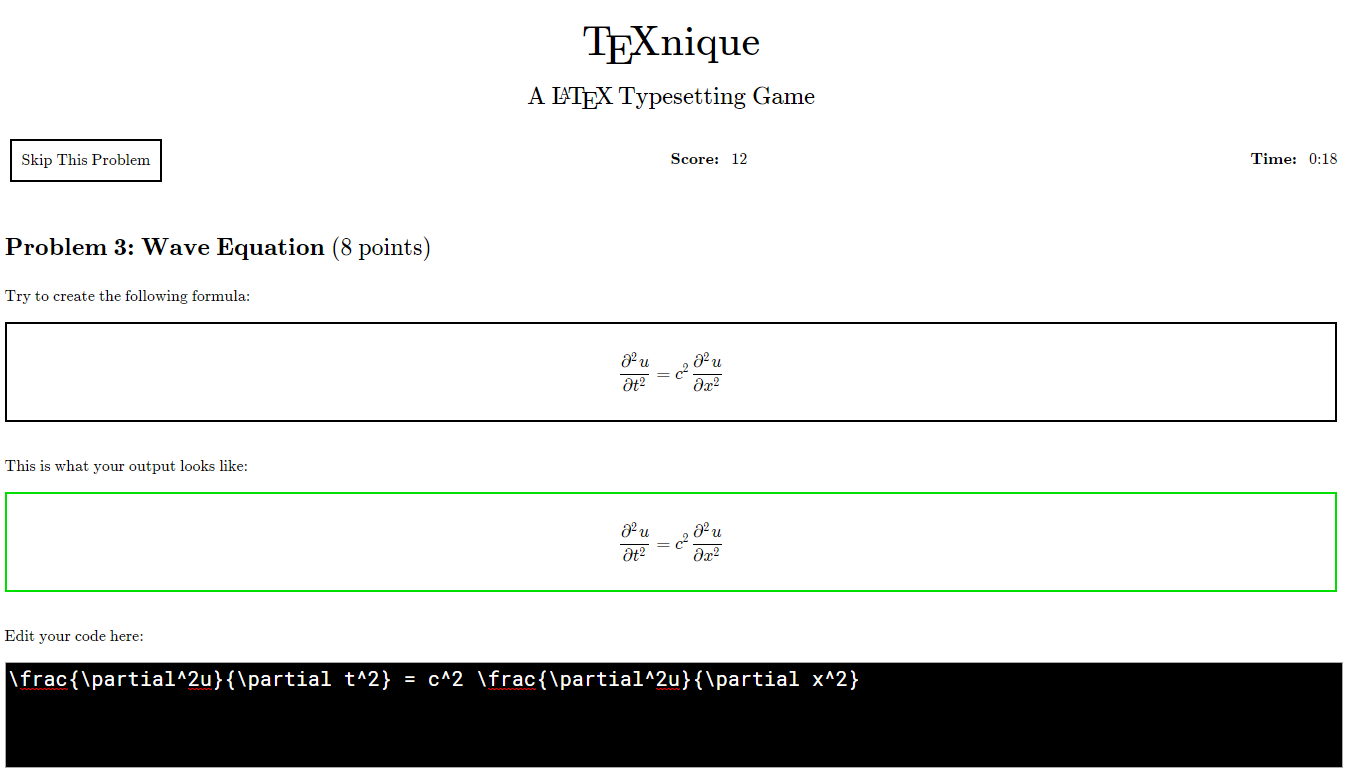
\includegraphics[width=1.0\linewidth,frame=]{./graphics/texnique.png}

% Caption is defined with a short and long version. The short version is shown in the 
% List of Figures section, and the long version is used directly with the figure. 			
	\caption[A screenshot of TeXnique, a game about typesetting equations.]{TeXnique, a game about typesetting equations \cite{texnique}. (Top) The game presents you with a rendered equation, (Bottom) the task is to enter LaTeX code that produces the same rendered equation. The green border on the lower rendering indicates it is a valid solution.}
	
% For figures label should be defined after the caption to ensure proper figure numbering.
	\label{fig:texnique}
\end{figure}